\documentclass[tikz,border=3.14mm]{standalone}
\usepackage{tikz}
\usepackage{physics}
\usetikzlibrary{shadings}

\begin{document}
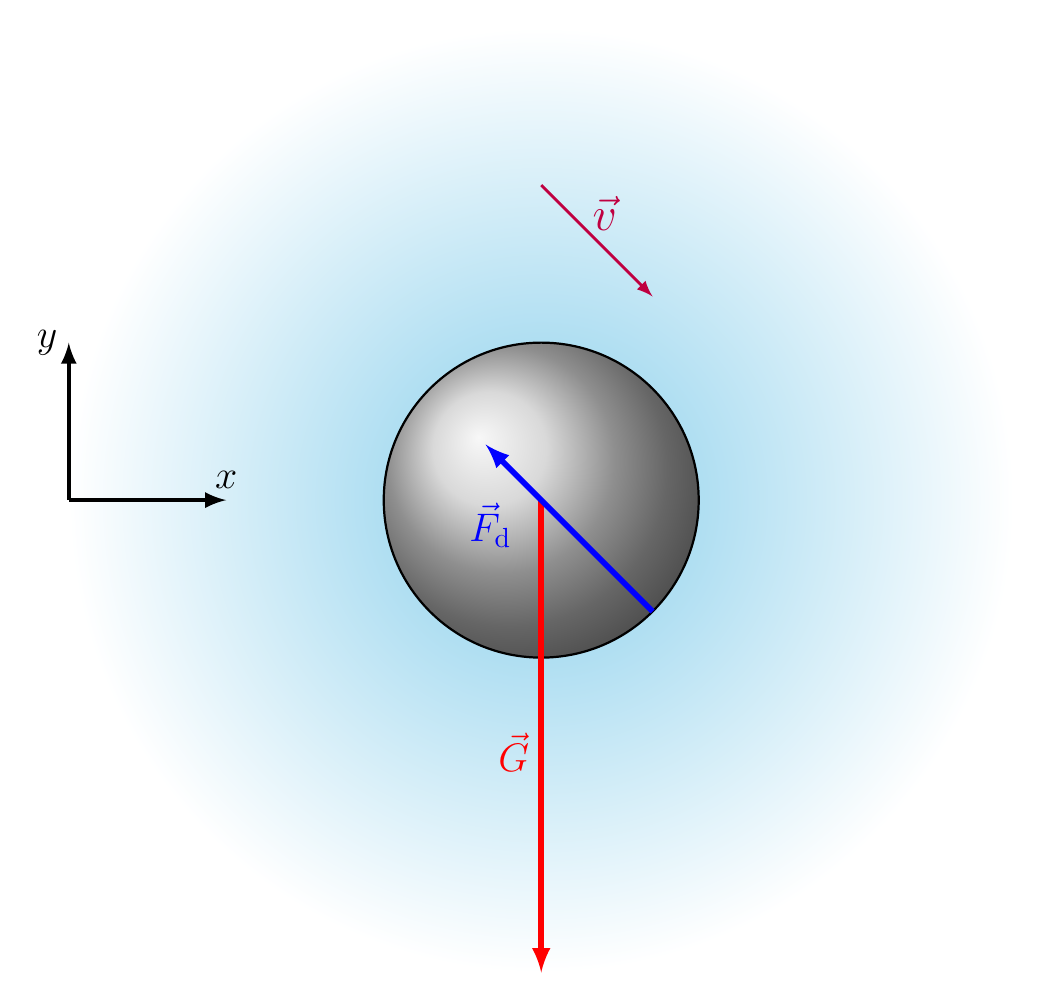
\begin{tikzpicture}[scale=2]

% Define forces
\def\gravityLength{3}
\def\velocityLength{1}
\def\resistanceLength{1.5}
\def\angle{-45}

% Define skyblue color
\definecolor{skyblue}{RGB}{135,206,235}

% Draw background as a sky
\shade[inner color=skyblue, outer color=white] (-3,-3) rectangle (3,3);

% Draw bullet as a shaded circle for a 3D effect
\shade[ball color=gray!40] (0,0) circle (1cm);

% Draw bullet outline to make it more visible
\draw[thick] (0,0) circle (1cm);

% Draw forces
\draw[-latex, line width=2pt, red] (0,0) -- (0,-\gravityLength) node[midway,left, yshift=-0.2cm] {\Large $\vec{G}$}; % Gravity

% Draw velocity at -45 degree angle outside the bullet
% \draw[-latex, line width=1pt, purple] (0,-\gravityLength-0.5) -- ++(-45:\velocityLength) node[midway,above, xshift=0.1cm] {\LARGE $\vec{v}$}; % Velocity
\draw[-latex, line width=1pt, purple] (0,+0.5*\gravityLength+0.5) -- ++(\angle:\velocityLength) node[midway,above, xshift=0.1cm] {\LARGE $\vec{v}$}; % Velocity
% Draw air resistance opposing velocity
\draw[-latex, line width=2pt, blue] (-45:1) -- ++(\angle + 180:\resistanceLength) node[midway,above,xshift=-1cm,yshift=-0.4cm] {\Large $\vec{F}_{\text{d}}$}; % Air Resistance

% Draw coordinate axes
\draw[-latex, ultra thick] (-3,0) -- (-2,0) node[above] {\Large $x$};
\draw[-latex, ultra thick] (-3,0) -- (-3,1) node[left] {\Large $y$};

\end{tikzpicture}
\end{document}
